\section{Method}
We use the Faster R-CNN model with ResNet50 as the backbone for our model. This is an object detection model, which consists of $2$ modules. The first module of the Faster R-CNN model is a deep fully convolutional network that proposes regions. The second module is a detector that uses proposed regions from the first one \cite{f-rcnn}. This is a single, unified network for object detection. By using the recently popular terminology of neural networks as the 'attention' mechanisms, the Region Proposal Networks (RPN) tells the Fast R-CNN where to look.

\begin{figure}[H]
\centering{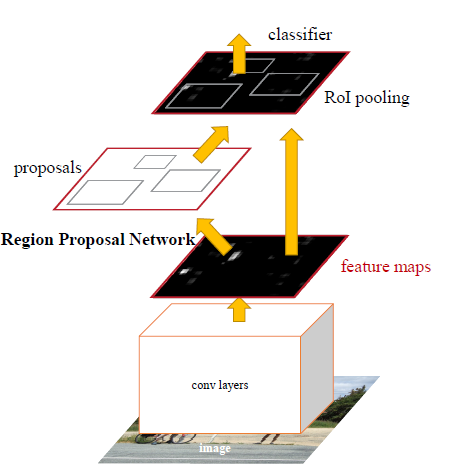
\includegraphics[scale=0.7]{faster-rcnn/faster-rcnn}}
\caption{Faster R-CNN is a single, unified network for object detection. The RPN module plays the role of the 'attention' of this network.}
\end{figure}

\subsection{Region Proposal Networks}
An RPN takes an image as input and outputs a set of rectangular object proposals each with an objectness score, which measures membership to a set of object classes. This process is modeled with a fully convolutional network. The structure of the RPN and an example are shown in Figure \ref{rpn}.

\begin{figure}[H]
\centering{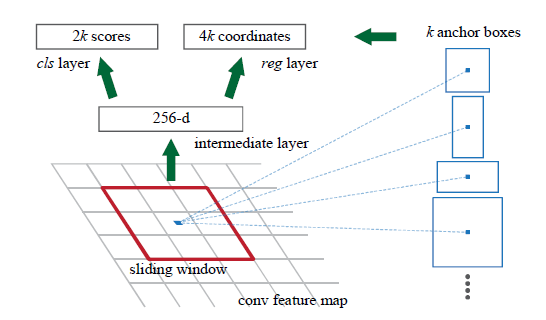
\includegraphics[scale=.8]{faster-rcnn/rpn}}
\caption{\textbf{Left:} RPN. \textbf{Right:} An example of detection using RPN.}
\label{rpn}
\end{figure}

\textbf{Loss function:} From \cite{f-rcnn}, the loss function of the RPN is:
$$L\left( {\left\{ {{p_i}} \right\},\left\{ {{t_i}} \right\}} \right) = \frac{1}{{{N_{cls}}}}\sum\limits_i {{L_{cls}}\left( {{p_i},p_i^*} \right) + \lambda \frac{1}{{{N_{reg}}}}\sum\limits_i {p_i^*} } {L_{reg}}\left( {{t_i},t_i^*} \right).$$

\subsection{Sharing Features for RPN and Fast R-CNN}
In the Faster R-CNN model, they use a 4-step training algorithm to learn shared features via alternating optimization. In the first step, the RPN is trained end-to-end by back-propagation and stochastic gradient descent (SGD). In the second step, they train a separate detection network by Fast R-CNN. In the third step, they use the detector network to initialize RPN training, and they let the two networks share convolutional layers. Finally, they keep the shared convolutional layers fixed, they fine-tune the unique layers of Fast R-CNN.
